%\documentclass[landscape,a0b,final,a4resizeable]{a0poster}
\documentclass[portrait,a0b,final]{a0poster}
%\documentclass[portrait,a0b,final,a4resizeable]{a0poster}
%\documentclass[portrait,a0b,final]{a0poster}
%%% Option "a4resizeable" makes it possible ot resize the
%   poster by the command: psresize -pa4 poster.ps poster-a4.ps
%   For final printing, please remove option "a4resizeable" !!

\usepackage{epsfig}
\usepackage{multicol}
\usepackage{pstricks,pst-grad}
\usepackage{amsmath}
\usepackage{setspace}
\usepackage{graphicx}
\usepackage{amsmath, amssymb}


%\usepackage{algorithm}
%\usepackage{algorithmic}



%%%%%%%%%%%%%%%%%%%%%%%%%%%%%%%%%%%%%%%%%%%
% Definition of some variables and colors
%\renewcommand{\rho}{\varrho}
%\renewcommand{\phi}{\varphi}
\setlength{\columnsep}{3cm}
\setlength{\columnseprule}{2mm}
\setlength{\parindent}{0.0cm}



%%%%%%%%%%%%%%%%%%%%%%%%%%%%%%%%%%%%%%%%%%%%%%%%%%%%
%%%               Background                     %%%
%%%%%%%%%%%%%%%%%%%%%%%%%%%%%%%%%%%%%%%%%%%%%%%%%%%%

\newcommand{\background}[3]{
  \newrgbcolor{cgradbegin}{#1}
  \newrgbcolor{cgradend}{#2}
  \psframe[fillstyle=gradient,gradend=cgradend,
  gradbegin=cgradbegin,gradmidpoint=#3](0.,0.)(1.\textwidth,-1.\textheight)
}



%%%%%%%%%%%%%%%%%%%%%%%%%%%%%%%%%%%%%%%%%%%%%%%%%%%%
%%%                Poster                        %%%
%%%%%%%%%%%%%%%%%%%%%%%%%%%%%%%%%%%%%%%%%%%%%%%%%%%%

\newenvironment{poster}{
  \begin{center}
  \begin{minipage}[c]{0.98\textwidth}
}{
  \end{minipage} 
  \end{center}
}



%%%%%%%%%%%%%%%%%%%%%%%%%%%%%%%%%%%%%%%%%%%%%%%%%%%%
%%%                pcolumn                       %%%
%%%%%%%%%%%%%%%%%%%%%%%%%%%%%%%%%%%%%%%%%%%%%%%%%%%%

\newenvironment{pcolumn}[1]{
  \begin{minipage}{#1\textwidth}
  \begin{center}
}{
  \end{center}
  \end{minipage}
}



%%%%%%%%%%%%%%%%%%%%%%%%%%%%%%%%%%%%%%%%%%%%%%%%%%%%
%%%                pbox                          %%%
%%%%%%%%%%%%%%%%%%%%%%%%%%%%%%%%%%%%%%%%%%%%%%%%%%%%

\newrgbcolor{lcolor}{0. 0. 0.80}
\newrgbcolor{gcolor1}{1. 1. 1.}
\newrgbcolor{gcolor2}{.80 .80 1.}

\newcommand{\pbox}[4]{
\psshadowbox[#3]{
\begin{minipage}[t][#2][t]{#1}
#4
\end{minipage}
}}



%%%%%%%%%%%%%%%%%%%%%%%%%%%%%%%%%%%%%%%%%%%%%%%%%%%%
%%%                myfig                         %%%
%%%%%%%%%%%%%%%%%%%%%%%%%%%%%%%%%%%%%%%%%%%%%%%%%%%%
% \myfig - replacement for \figure
% necessary, since in multicol-environment 
% \figure won't work

\newcommand{\myfig}[3][0]{
\begin{center}
  \vspace{1.5cm}
  \includegraphics[width=#3\hsize,angle=#1]{#2}
  \nobreak\medskip
\end{center}}



%%%%%%%%%%%%%%%%%%%%%%%%%%%%%%%%%%%%%%%%%%%%%%%%%%%%
%%%                mycaption                     %%%
%%%%%%%%%%%%%%%%%%%%%%%%%%%%%%%%%%%%%%%%%%%%%%%%%%%%
% \mycaption - replacement for \caption
% necessary, since in multicol-environment \figure and
% therefore \caption won't work

%\newcounter{figure}
\setcounter{figure}{1}
\newcommand{\mycaption}[1]{
  \vspace{0.5cm}
  \begin{quote}
    {{\sc Figure} \arabic{figure}: #1}
  \end{quote}
  \vspace{1cm}
  \stepcounter{figure}
}



%%%%%%%%%%%%%%%%%%%%%%%%%%%%%%%%%%%%%%%%%%%%%%%%%%%%%%%%%%%%%%%%%%%%%%
%%% Begin of Document
%%%%%%%%%%%%%%%%%%%%%%%%%%%%%%%%%%%%%%%%%%%%%%%%%%%%%%%%%%%%%%%%%%%%%%

\begin{document}

\background{1. 1. 1.}{1. 1. 1.}{0.5}

\vspace*{2cm}


\newrgbcolor{lightblue}{0. 0. 0.80}
\newrgbcolor{white}{1. 1. 1.}
\newrgbcolor{whiteblue}{.80 .80 1.}


\begin{poster}

%%%%%%%%%%%%%%%%%%%%%
%%% Header
%%%%%%%%%%%%%%%%%%%%%
\begin{center}
\begin{pcolumn}{0.98}

\pbox{0.962\textwidth}{}{linewidth=2mm,framearc=0.3,linecolor=lightblue,fillstyle=gradient,gradangle=0,gradbegin=white,gradend=whiteblue,gradmidpoint=1.0,framesep=1em}{

%%% Unisiegel
\begin{minipage}[c][9cm][c]{0.1\textwidth}
  \begin{center}
    \includegraphics[angle=0,width=8cm]{images/hamilton-logo.epsi}
  \end{center}
\end{minipage}
%%% Titel
\begin{minipage}[c][9cm][c]{0.78\textwidth}
  \begin{center}
    {\sc \Huge Of queues and cures: A solution to modelling the inter time arrivals of cloud outage events}\\[10mm]
    {\Large Jonathan Dunne, David Malone\\[7.5mm]
    Hamilton Institute, Maynooth University.}
  \end{center}
\end{minipage}
%%% GK-Logo
\begin{minipage}[c][9cm][c]{0.1\textwidth}
  \begin{center}
    \includegraphics[width=7cm,angle=0]{MULogo.eps}
  \end{center}
\end{minipage}

}
\end{pcolumn}
\end{center}


\vspace*{2cm}



%%%%%%%%%%%%%%%%%%%%%
%%% Content
%%%%%%%%%%%%%%%%%%%%%
\begin{center}
\begin{pcolumn}{0.49}
\pbox{0.9\textwidth}{28cm}{linewidth=2mm,framearc=0.1,linecolor=lightblue,fillstyle=gradient,gradangle=0,gradbegin=white,gradend=white,gradmidpoint=1.0,framesep=1em}{
\medskip
%%% Abstract
\begin{center}\pbox{0.8\textwidth}{}{linewidth=2mm,framearc=0.1,linecolor=lightblue,fillstyle=gradient,gradangle=0,gradbegin=white,gradend=whiteblue,gradmidpoint=1.0,framesep=1em}{\begin{center}Background \& Introduction\end{center}}\end{center}\vspace{1.25cm}

Background: 

\medskip 
\medskip 

\begin{itemize}
\item Cloud outages come from multiple sources,
\item High volume outages are a challenge for SME's,
\item Which distribution can be used to model these events,
\item If a distribution is known model development can follow.
\end{itemize}

\medskip
\medskip


Aim: understand which distribution can model outage events.

\medskip 
\medskip 

Complication: Outage events are highly dispersed.

\medskip 

\begin{itemize}
\item Test for Goodness of Fit,
\item Check against known distributions,
\item Distributions include: lognormal, gamma, Weibull,
\item exponential, logistic, loglogistic and Pareto.
\end{itemize}


}
\end{pcolumn}
%%%%%%%%%%%%%%%%%%%%%%
%%%%%%%%%%%%%%%%%%%%%%
\begin{pcolumn}{0.49}
\pbox{0.9\textwidth}{28cm}{linewidth=2mm,framearc=0.1,linecolor=lightblue,fillstyle=gradient,gradangle=0,gradbegin=white,gradend=white,gradmidpoint=1.0,framesep=1em}{

\medskip
%%% Introduction
\begin{center}\pbox{0.8\textwidth}{}{linewidth=2mm,framearc=0.1,linecolor=lightblue,fillstyle=gradient,gradangle=0,gradbegin=white,gradend=whiteblue,gradmidpoint=1.0,framesep=1em}{\begin{center}Dataset\end{center}}\end{center}\vspace{1.25cm}

\smallskip

The study examines 250 cloud outage events from a large enterprise system.

\medskip 
\medskip 

\begin{itemize}
\item Study looked at the inter arrival times of each outage,
\item Data was collected over a 12 month period (January - December),
\item The software running on this enterprise system was developed in Java,
\item Developers follow a Continuous Delivery development model.
\end{itemize}

\medskip 
\medskip 

Our key research question:

\medskip 
\medskip 

\begin{itemize}
\item Which distribution can best model the inter arrival time of cloud outage events.
\end{itemize}


\smallskip


}
\end{pcolumn}
%%%%%%%%%%%%%%%%%%%%%%
\end{center}
%%%%%%%%%%%%%%%%%%%%%%

%%%%%%%%%%%%%%%%%%%%%%%%%%%%%%%%%%%%%%%%%%%%%%%%%%%%%%%%%%%%%%%%%%%%%%%%
% ROW 2                                                                %
%%%%%%%%%%%%%%%%%%%%%%%%%%%%%%%%%%%%%%%%%%%%%%%%%%%%%%%%%%%%%%%%%%%%%%%%
\vspace*{2cm}

%%%%%%%%%%%%%%%%%%%%%
%%% Content
%%%%%%%%%%%%%%%%%%%%%
\begin{center}
\begin{pcolumn}{0.49}
\pbox{0.9\textwidth}{28cm}{linewidth=2mm,framearc=0.1,linecolor=lightblue,fillstyle=gradient,gradangle=0,gradbegin=white,gradend=white,gradmidpoint=1.0,framesep=1em}{

\medskip
%%% Introduction
\begin{center}\pbox{0.8\textwidth}{}{linewidth=2mm,framearc=0.1,linecolor=lightblue,fillstyle=gradient,gradangle=0,gradbegin=white,gradend=whiteblue,gradmidpoint=1.0,framesep=1em}{\begin{center}Analysis \& Discussion\end{center}}\end{center}\vspace{1.25cm}

\smallskip

Method:

\medskip
\medskip

\begin{itemize}
\item Model the parameters of each distribution using the R fitdistrplus library,
\item Test the GoF characteristics of each distribution using the ADGofTest library.
\end{itemize}

\medskip
\medskip



\begin{center}
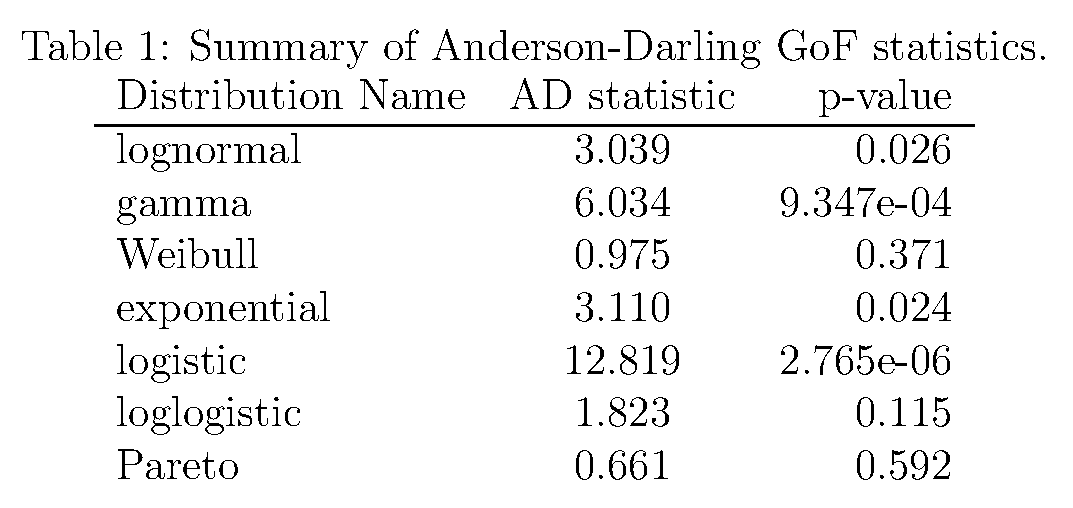
\includegraphics[width=30cm]{table1}
\end{center}


}
\end{pcolumn}
%%%%%%%%%%%%%%%%%%%%%%
\begin{pcolumn}{0.49}
\pbox{0.9\textwidth}{28cm}{linewidth=2mm,framearc=0.1,linecolor=lightblue,fillstyle=gradient,gradangle=0,gradbegin=white,gradend=white,gradmidpoint=1.0,framesep=1em}{

\medskip
%%% Introduction
\begin{center}\pbox{0.8\textwidth}{}{linewidth=2mm,framearc=0.1,linecolor=lightblue,fillstyle=gradient,gradangle=0,gradbegin=white,gradend=whiteblue,gradmidpoint=1.0,framesep=1em}{\begin{center}Results: Histogram \& Quantiles\end{center}}\end{center}\vspace{1.25cm}

\smallskip

\begin{center}
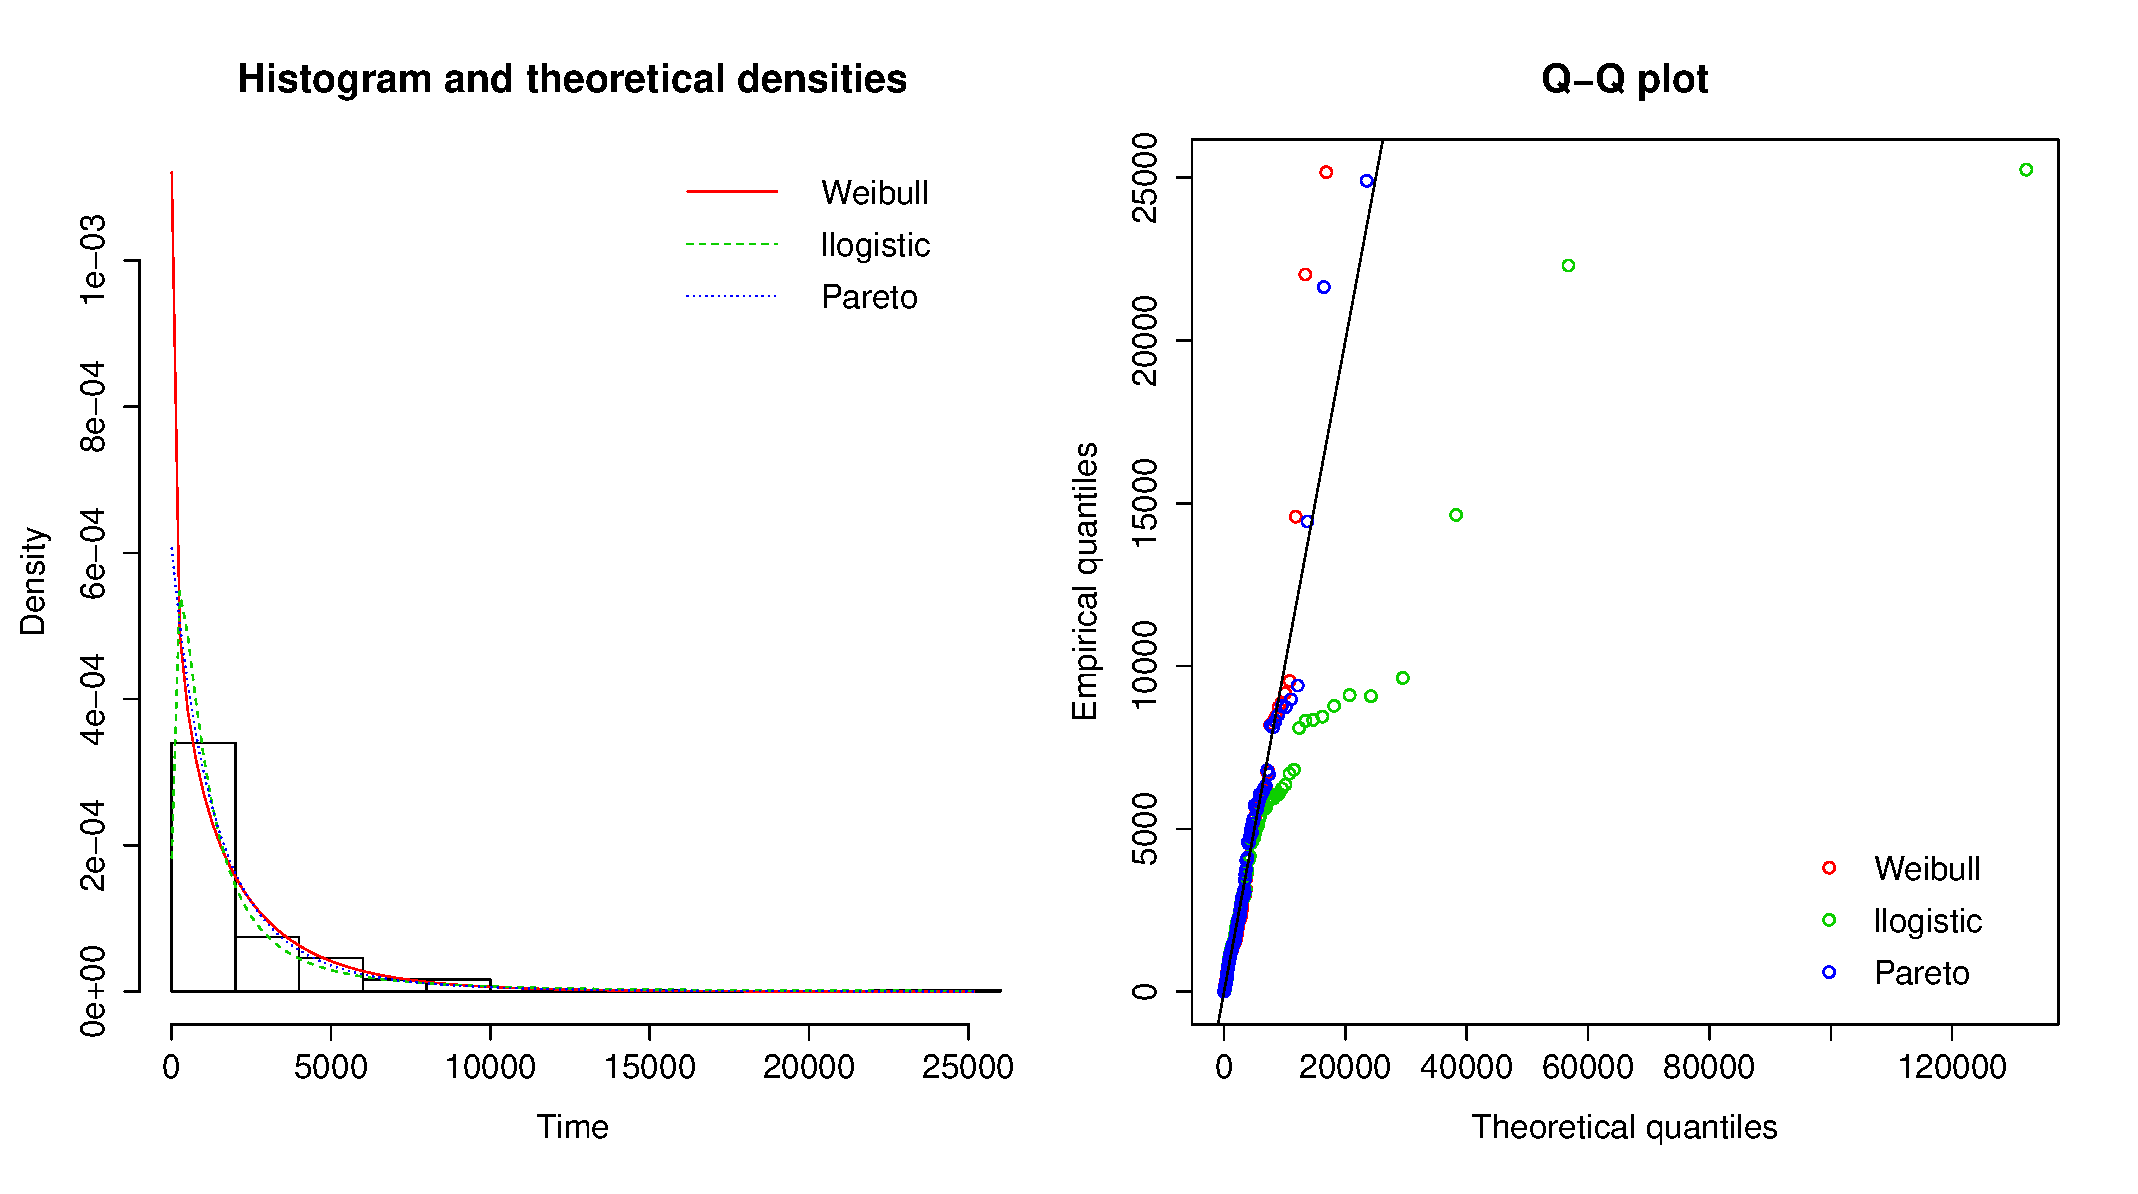
\includegraphics[width=33cm]{graph1}
\end{center}


}
\end{pcolumn}
%%%%%%%%%%%%%%%%%%%%%%
\end{center}
%%%%%%%%%%%%%%%%%%%%%%%%%%%%%%%%%%%%%%%%%%%%%%%%%%%%%%%%%%%%%%%%%%%%%%%%
% ROW 3                                                                %
%%%%%%%%%%%%%%%%%%%%%%%%%%%%%%%%%%%%%%%%%%%%%%%%%%%%%%%%%%%%%%%%%%%%%%%%
\vspace*{2cm}

%%%%%%%%%%%%%%%%%%%%%
%%% Content
%%%%%%%%%%%%%%%%%%%%%
\begin{center}
\begin{pcolumn}{0.49}
\pbox{0.9\textwidth}{28cm}{linewidth=2mm,framearc=0.1,linecolor=lightblue,fillstyle=gradient,gradangle=0,gradbegin=white,gradend=white,gradmidpoint=1.0,framesep=1em}{

\medskip
%%% Introduction
\begin{center}\pbox{0.8\textwidth}{}{linewidth=2mm,framearc=0.1,linecolor=lightblue,fillstyle=gradient,gradangle=0,gradbegin=white,gradend=whiteblue,gradmidpoint=1.0,framesep=1em}{\begin{center}Results: CDF \& Probabilities\end{center}}\end{center}\vspace{1.25cm}

\smallskip

\begin{center}
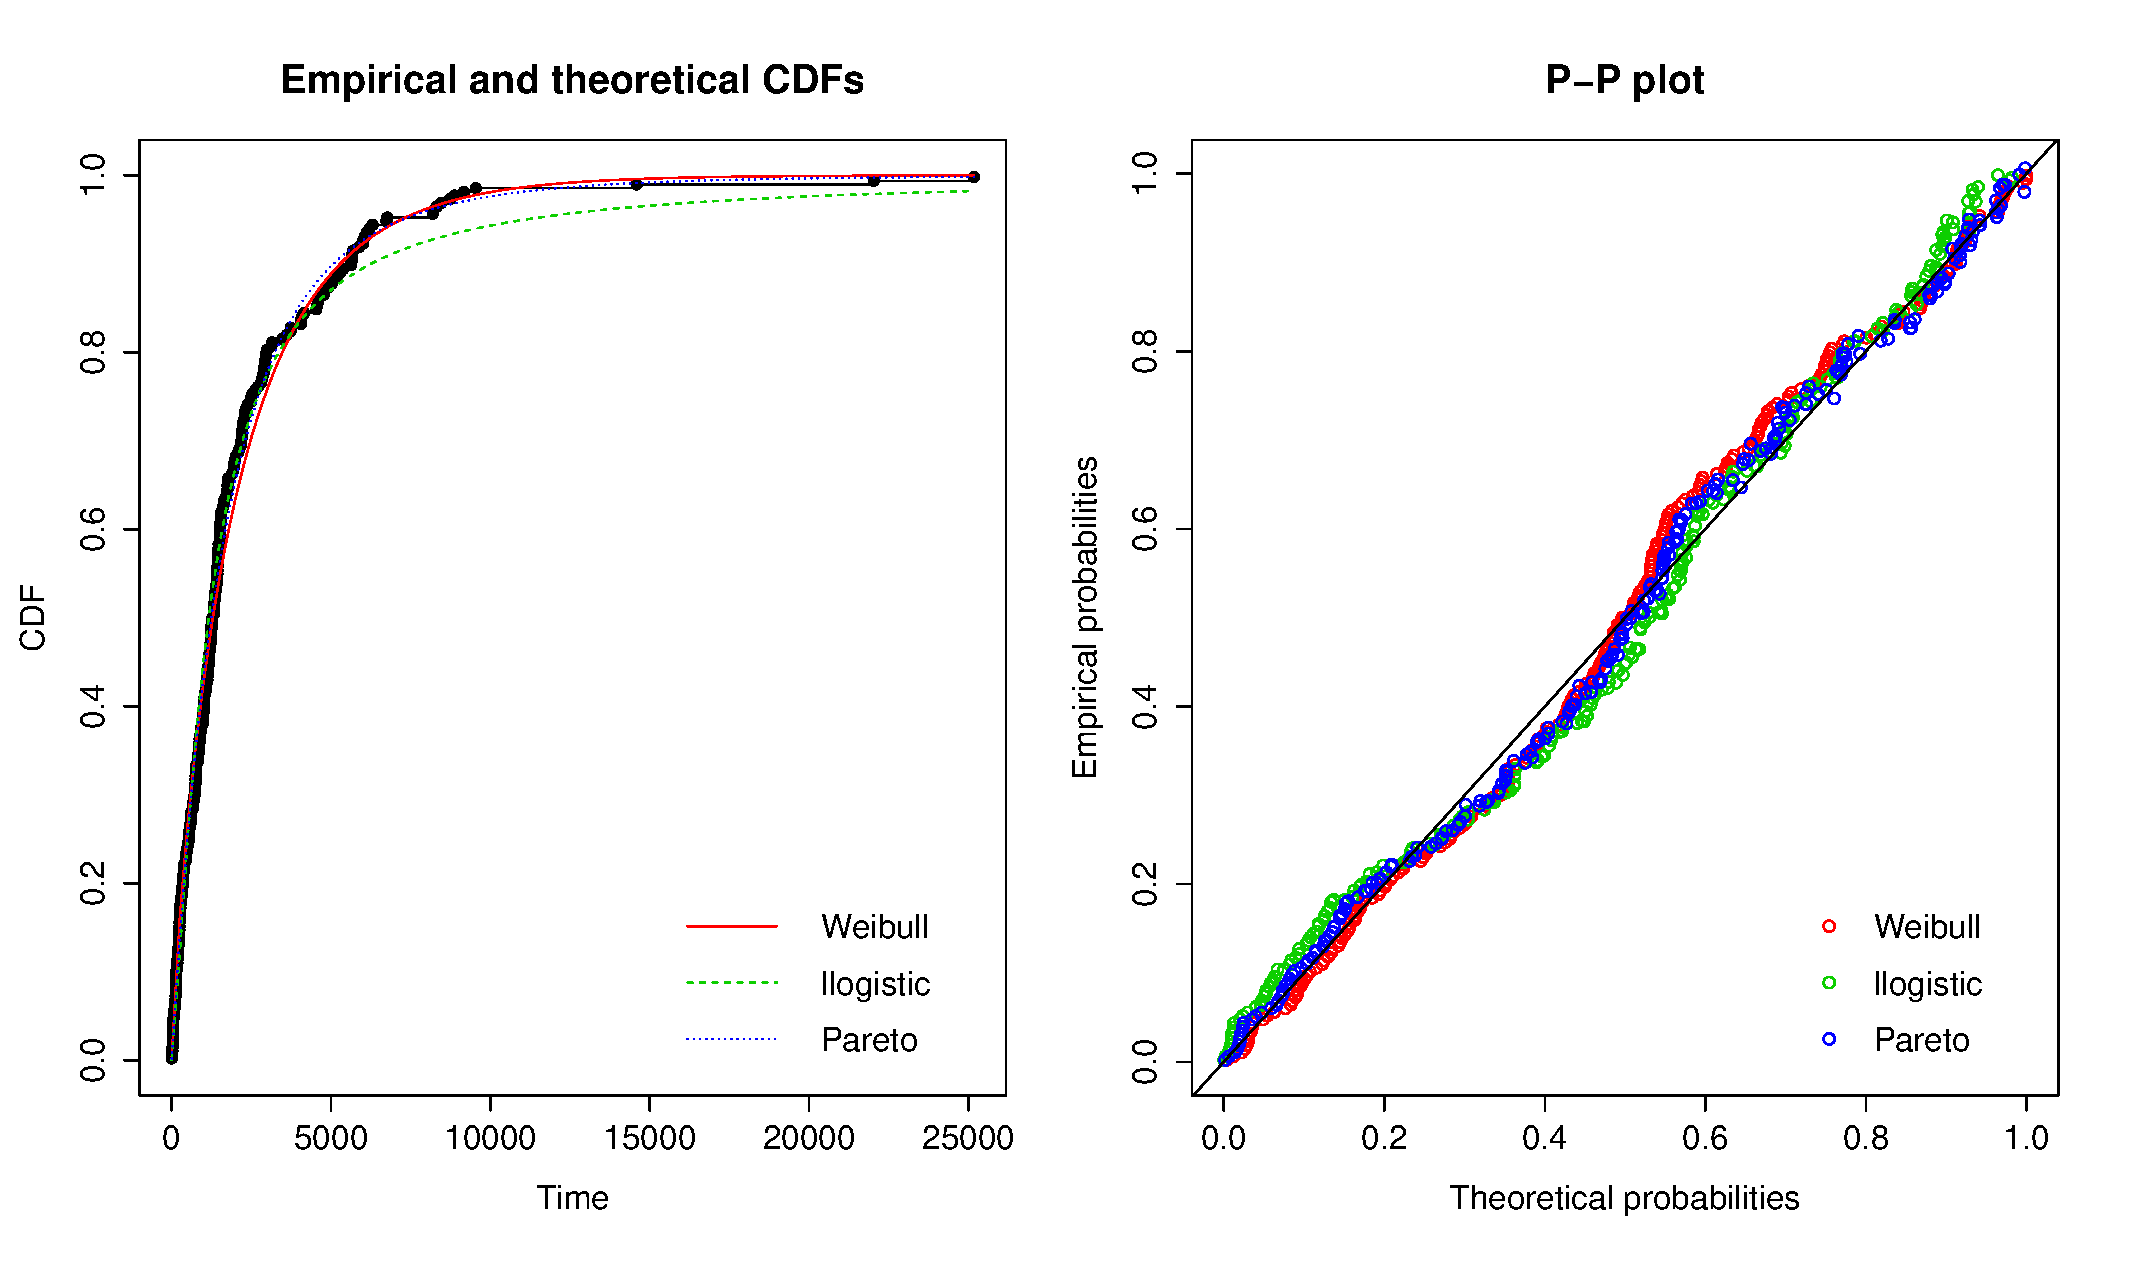
\includegraphics[width=33cm]{graph2}
\end{center}


}
\end{pcolumn}
%%%%%%%%%%%%%%%%%%%%%%
\begin{pcolumn}{0.49}
\pbox{0.9\textwidth}{28cm}{linewidth=2mm,framearc=0.1,linecolor=lightblue,fillstyle=gradient,gradangle=0,gradbegin=white,gradend=white,gradmidpoint=1.0,framesep=1em}{

\medskip
%%% Introduction
\begin{center}\pbox{0.8\textwidth}{}{linewidth=2mm,framearc=0.1,linecolor=lightblue,fillstyle=gradient,gradangle=0,gradbegin=white,gradend=whiteblue,gradmidpoint=1.0,framesep=1em}{\begin{center}Conclusions, Future and Related Work\end{center}}\end{center}\vspace{1.25cm}

\smallskip

Conclusions:
\begin{itemize}
\item The Pareto distribution is an effective distribution for modelling the interarrival times of cloud outages.
\item Result can be used as an arrival time parameter for a queuing model.
\end{itemize}

\medskip

Future Work:
\begin{itemize}
\item Establish service time distribution.
\item Queue simulation of inter arrival and service time distributions.
\end{itemize}

\medskip

Related work:
\begin{itemize}
\item \emph{Web Page https://cran.r-project.org/web/packages/fitdistrplus/index.html}, Delignette-Muller, M.L. and Dutang, C. and Pouillot, R. and Denis, 2015

\item \emph{Web Page https://cran.r-project.org/web/packages/ADGofTest/index.html}, Bellosta, C.J.G 2011
\end{itemize}

}
\end{pcolumn}
\end{center}

\end{poster}

\end{document}

